%!TEX root = ../thesis.tex
%\input{commands.tex}
%*******************************************************************************
%****************************** Third Chapter **********************************
%*******************************************************************************
\chapter{Haplotype phasing consistency as a signal for physical linkage in scaffolding and assembly}

% **************************** Define Graphics Path **************************
\ifpdf
    \graphicspath{{Chapter4/Figs/Raster/}{Chapter4/Figs/PDF/}{Chapter4/Figs/}}
\else
    \graphicspath{{Chapter4/Figs/Vector/}{Chapter4/Figs/}}
\fi



\section{Background}
\par{
Reference genomes have enabled a range of genomic analysis by providing prior knowledge of the sequence 
and giving genomic context as well as a common coordinate system by which to compare multiple genomes \cite{1000genomes} \cite{GRCh38}. Assembling reference genomes is complicated by repetitive sequences, heterozygosity, and sequencing errors. As discussed in Chapter 3, when an assembly encounters inexact homologous sequences, it must determine which of these cases the sequence differences are due to. 
If the assembler cannot distinguish between heterozygosity and repeats, and if no reads span the homologous sequence into more unique regions, the contig must end
to avoid assembly distant regions or sequence from different chromosomes together. Historically reference genomes were created by large haploid bacterial artificial chromosomes (BACs) clone libraries \cite{human}. 
These methods overcame much of the problem of resolving repeats and heterozygosity because of their length allowing them to read through all but the longest segmental duplications and the fact that they are inherently haploid. However, because each of these BACs were sequenced with Sanger sequencing and assembled, they were still subject to problems in repeats longer than the Sanger reads that were close enough to one another to occur in the same BAC clone. But most importantly, these methods are far too costly to apply to many genomes. 
}

\par{
More recently the cost reductions of long read technologies \cite{pacbio} \cite{oxford}, and reduced error profiles through optimization of the circular consensus method \cite{ccs}\cite{HIFI}
as well as the emergence of other long range genetic information technologies \cite{10xlinked} \cite{HiC} \cite{bionano} 
have converged to make high quality, cost effective reference genomes. This has then resparked interest in assembly 
as well as large reference generation projects. Efforts have begun on the Earth Biogenome Project (EBP)\cite{EBGP}, a global project to sequence the entire diversity of multicellular eukaryotic life. In the UK, the Sanger Institute and partners have started to sequence 60,000 species from the British Isles in the Darwin Tree of Life (DToL) project. These projects aim to provide a scientific resource for the next generation of biological science, for environmental conservation, and to study evolution at a much broader and deeper scale than ever before. 
}

\par{
As discussed in Chapter 3, one of the primary remaining difficulties in assembling reference quality genomes is high levels of heterozygosity such as found in many of the non-model organisms included in the EBG and DToL projects. While Chapter 3 focused on going from a pool of individuals---and thus many haplotypes---to a single individual---and thus two haplotypes, this chapter focuses on the problems encountered with high levels of heterozygosity within an individual and the improvements that can be made computationally to both alleviate those problems as well as use the high levels of heterozygosity to our advantage. 
For these newer technologies mentioned above, there are now assembly algorithms that deal with each data type \cite{falcon} \cite{supernova} \cite{bionano_assembly} 
as well as combinations of multiple technologies \cite{genemyers} \cite{hybrid10x} \cite{hicscafffirst}\cite{hicassembly}. 
 These methods try to co-assemble both haplotypes arriving at a haploid consensus \cite{watchtower} \cite{canu} 
 or a diploid assembly \cite{falconPHASE} \cite{supernova} \cite{hifiasm}\cite{dipasm}, but heterozygosity still injects complexity and ambiguity on top of a haploid assembly process.
}

\par{
As mentioned in Chapter 3, one method for dealing with the problem of heterozygosity is inbreeding organisms to a point of low heterozygosity \cite{drosophila}, 
but this is not possible for all organisms. Trio-sga used pedigree sequencing information in the assembly algorithm \cite{trio-sga} 
but was built for short reads and does not work on long read data. Recently Koren et al. described trio binning which uses a mother-father-child trio to 
separate long reads into their haplotype of origin prior to haploid assembly \cite{triobinning}. 
While this method is very effective, creating such a cross would be infeasible for many species and costly for the vast number of reference genomes these projects intend to sequence. 
Another recent approach using the new highly accurate HIgh FIdelity (HIFI) ccs reads from PacBio along with homopolymer compression and other methods to reduce errors dramatically is to 
require nearly identical sequence similarity to extend the assembly graph \cite{HICANU}. This results in the haplotypes being b v separately in all but the few long stretches of homozygosity in 
a genome. They then run a haplotic purging software PurgeDups \cite{purgedups} to remove one of the haplotype assemblies. This has the downside of not matching the haplotypes to make comparisons, but that could be done 
fairly well as an additional analysis step. This method does not explicitly phase the haplotypes and may have long phase switches especially across long regions of homozygosity.
}

\par{
Despite the incredible advances made over the past several years in both sequencing technologies and assembly methods, we still cannot assemble whole chromosomes or chromosome arms with a 
single technology for most organisms. After assembly we are left with some level of fragmentation of chromosomes into contiguous sequences (contigs) which we wish to scaffold together. While the 
PacBio HIFI technology has many wonderful properties including continuous, highly accurate reads, it does not produce long enough reads to span many repeat or low sequence complexity regions in most genomes.
 10x Genomics linked read technology, however, will create barcode linked short reads across much longer molecules (50kb+) with some molecules reaching well over 250kb \cite{10xlinked}. Optical map technology in which the DNA is linearized and flourescent markers are attached to sequence specific loci via restriction digestion and optically inspected can give sparse data for pieces of DNA about as long as can be isolated with modern high molecular weight extraction methods\cite{opticalmaps1}. And high-throughput chromatin conformation capture sequencing (Hi-C) data creates links between sequences physically located close to one another. And while there will be cross-chromosomal links, the large majority of links are intra-chromosomal but can create links of almost any length \cite{3CHIC} \cite{HIC}. Each of these technologies have been used to break misassemblies in contigs and scaffold contigs\cite{scaff10x}\cite{opticalhuman}\cite{hicscafffirst}\cite{SALSA}\cite{GRAAL}\cite{instaGRAAL}. But some of these scaffolders have been known to introduce misassemblies \cite{hicscafffirst}. 
}


\par{
While high levels of heterozygosity make the assembly problem harder for traditional methods, haplotype phasing consistency (reads containing multiple heterozygous alleles segregate into two---if diploid---groups according to which alleles they have) can be used as a signal of physical linkage in both assembly and scaffolding and as a method to differentiate inexact repeats from haplotype differences. While the conventional thinking is that heterozygosity makes these problems more difficult, we turn this around and use the phasing consistent property of heterozygous sites as a powerful way to simplify and add statistical power to them. In this chapter we present a toolkit for phasing, phasing aware assembly, and phasing aware scaffolding called phasstools (PHasing and ASSembly tools). It is made up of a number of github repositories with a master repository to give a unified command line interface. The code is open source and available at https://github.com/wheaton5/phasstools and the submodule repositories which are linked from the main repository. The use cases are reference based and fully de novo haplotype phasing, assembly based phasing aware scaffolding, and phasing aware assembly. While I will show results from the phasing aware assembly, these are preliminary and not without problems, which I will discuss. For that reason, I will first address the steps required to use phasing consistency for highly accurate assembly scaffolding. First I will outline phasing consistency, then introduce heterozygous single nucleotide polymorphism (SNP) kmer pairs as a mechanism for \textit{de novo} haplotype phasing. Next I introduce an algorithm for \textit{de novo} haplotype phasing using sparse \textit{Bernoulli} mixture model clustering---an algorithm very similar to the clustering algorithm used in Chapter 2. I discuss some several benefits and limitations of this algorithm for our purposes. I then move on to another phasing algorithm based on a given assembly to that can be used for phasing aware scaffolding. We show results for both phasing algorithms on a dataset from the Darwin Tree of Life program from the butterfly \textit{Vanessa atalanta}. Next we consider haploid sex contig detection, because these contigs will need to be treated differently in the steps going forward. Before scaffolding, we discuss breaking contigs that are incorrectly joined in a chimeric misassembly using Hi-C linkage information and the phasing consistency of those links across the midpoint of a moving window. Finally, we discuss phasing aware scaffolding and the results on \textit{Vanessa atalanta} HiCanu assembly. We then continue by discussing the incomplete phased assembly process. 
}


\section{Phasing aware scaffolding of an existing assembly: phasst scaff}

\par{
Our goal is to use the phasing consistency of Hi-C reads and optionally linked reads that cover heterozygous sequence on two contigs. First we must find those heterozygous sites. Then we can define phasing consistency of those sites.
}


\subsection{Paired heterozygous SNP kmers}
\par{
In the case of scaffolding an existing assembly, we could map the reads to the assembly and call variants to find heterozygous sites as is the common workflow for resequencing efforts. In an effort to be unbiased by the 
assembly, and to be general to a de novo assembly process, we will use paired SNP kmers---kmers that vary only in the middle base and that have counts that are roughly half of the homozygous kmer counts. We generate the 
kmer count spectra with a fast disk backed kmer counter KMC \cite{kmc}\cite{kmc2}\cite{kmc3}. Figure \ref{figure:kmc} shows an example kmer count histogram. 
}

\begin{figure}[htbp!]

\caption{Kmer count spectra and heterozygous paired kmers}
\label{figure:kmc}
\begin{centering}
\includegraphics[width=0.65\textwidth]{kmc.png}
\par{An example of kmer count spectra showing error kmers on the left, heterozygous kmers in the first peak and homozygous kmers in the next peak.}
\end{centering}
\end{figure}

\par{
We then use the heterozygous range of the kmer spectra with code from purge dups, a tool for removing sequences from assemblies when multiple haplotypes were assembled separately\cite{purgedups}. The kmers are then dumped in alphabetical order and we search for pairs of kmers which vary in only the middle base and fall into the heterozygous counts range. We give a further restriction that the sum of the counts of the kmers with the other two possible bases in the middle are not high as sequences with very high repeat count can produce, through sequencing error or mutations, two kmers in these counts range with the middle base altered. It should also be noted, that while I generally refer to these kmer pairs as heterozygous kmer pairs, they may also represent paralogous kmer pairs. We will use the phasing consistency of these kmer pairs with each other to determine if they are more likely to be from heterozygosity or paralogous sequences. Each produces a characteristic pattern in the kmer consistency counts.
}

\subsection{Read data kmer information}
\par{
We will use the kmers in the reads to determine if heterozygous paired kmers are phasing consistent with other paired kmers. So we go through the reads of each long range genetic information including HiC, PacBio, linked reads, and nanopore and store the position and ID of each paired kmer on the reads. We then store this on disk in a custom binary format for later use. Of note here is that the linked read technology may have multiple molecules per barcode whereas in other technologies, reads represent single physically linked molecules. Richard Durbin has developed a method to \textit{de novo} assign reads from barcodes to molecule groups using shared kmers across barcode sets to cluster reads into their molecules of origin. In this work, we choose not to use this as it is unpublished and not extensively tested. Instead, we use the distance on the assembly contigs to determine which reads came from which barcode. With the recommended DNA input, high molecular weight (HMW) extraction sizes, and number of partitions, we expect the poisson loading to result in a mean of roughly ten molecules per barcode. Because the total amount of DNA per partition is a small percentage of the total genome sizes we work with, the chances of a partition having molecules which arose from nearby or overlapping locations is rare. Thus we can deduce that reads from a barcode which map close to one another on a reference or assembly arose from the same HMW molecule. While this is not fully \textit{de novo}, it is highly unlikely to cause a false inference because a chimeric misassembly causing incorrect linked read molecule inference would not result in a phasing consistent signal.
}

\begin{figure}[htbp!]
\caption{Identify paired kmer location in long range genetic data}
\label{figure:techs}
\begin{centering}
\includegraphics[width=0.65\textwidth]{techs.png}
\par{Different data types used. Top left: PacBio, Top right: Hi-C, Bottom left: nanopore, Bottom right: Linked reads}
\end{centering}
\end{figure}
\subsection{Phasing consistency}
\par{
For each kmer pair, we refer to one as the reference allele and one as the alternate allele arbitrarily without loss of generality. We go through the read kmer data and for every pairwise kmer on the molecule, we update counts for their associated heterozygous paired kmers. If the read contains the reference version of paired kmer k1 and reference version of paired kmer k2, the cis1 count gets incremented. We may do this with any of the data types for different purposes, but we do not combine counts across data types as the error modes may be different. For example, the Hi-C data will have some spurious connections across chromosomes due to the 3D conformation of the chromosomes in a particular nucleus. For the linked reads, we may also stipulate that a version of paired kmer k1 and paired kmer k2 be within some distance of each other on the assembly.
}
\subsubsection{Pairwise haplotype phasing consistency}



\begin{figure}[htbp!]
\caption{Pairwise phasing consistency counts}\label{figure:consistency}
\centering
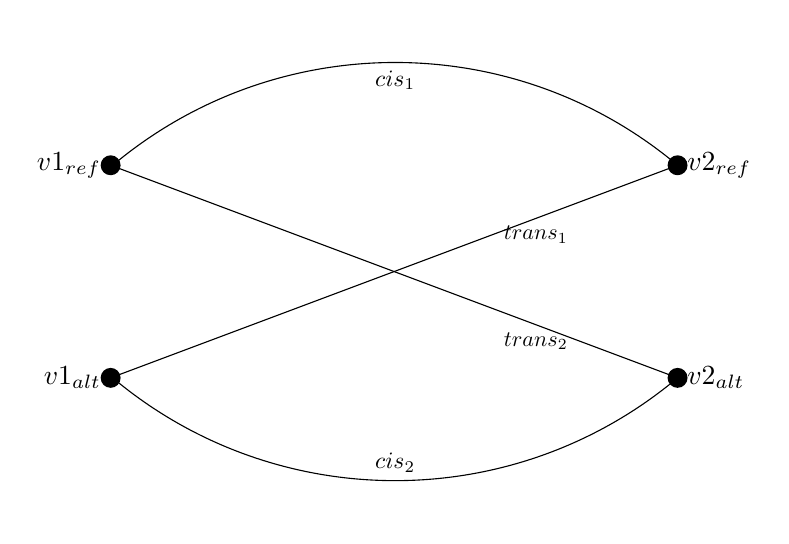
\begin{tikzpicture}[scale=1.8]
\def\xoffset{0}
\def\yoffset{0}
\def\titley{1.2}
\def\panellength{5}
\def\titlescale{1}
 \def\subtitlescale{0.7}
 \node[anchor=east] at (0 + \xoffset,2 + \yoffset) {$v1_{alt}$};
\draw (4 + \xoffset,2 + \yoffset) arc (-50:-130:3.1) node[midway,above, scale=0.85] {$cis_2$};
\fill (0 + \xoffset ,2 + \yoffset) circle[radius=2pt];
\node[anchor=west] at (4 + \xoffset,2 + \yoffset) {$v2_{alt}$};
\fill (4 + \xoffset,2 + \yoffset) circle[radius=2pt];
\node[anchor=east] at (0 + \xoffset,3.5 + \yoffset) {$v1_{ref}$};
\fill (0 + \xoffset,3.5 + \yoffset) circle[radius=2pt];
\draw (4 + \xoffset,3.5 + \yoffset) arc (50:130:3.1) node[midway,below, scale=0.85]{$cis_1$};
\draw (4 + \xoffset ,3.5 + \yoffset) -- node[below, scale=0.8] {$trans_1$} (2 + \xoffset,2.75 + \yoffset) -- (0+ \xoffset,2 + \yoffset);
\draw (4 + \xoffset,2 + \yoffset) -- node[below, scale=0.8] {$trans_2$} (2+ \xoffset,2.75 + \yoffset) -- (0+ \xoffset,3.5 + \yoffset);
\node[anchor=west] at (4+ \xoffset,3.5 + \yoffset) {$v2_{ref}$};
\fill (4+ \xoffset,3.5 + \yoffset) circle[radius=2pt];
\end{tikzpicture}
\par{
We denote one of each kmer pair as the reference or alternative arbitrarily. Molecules that have the sequences of one of the kmers from each of two kmer pairs will fall into one of four cases represented here by the four edges in this graph. We calculate the counts of molecules falling into each of these four categories. Phasing consistent heterozygous kmer pairs will have counts predominantly on both cis edges or both trans edges.
}
\end{figure}

\subsubsection{Phasing consistency and error modes}

\par{
There are several distinctive signals we can see from pairwise phasing consistency counts and further insight can be gained when looking at those phenotypes across the multiple paired kmers for which a given paired kmer will have data.
}

\begin{figure}[htbp!]
\caption{Pairwise phasing consistency counts}\label{figure:consistency2}
\centering
\sidesubfloat[]{
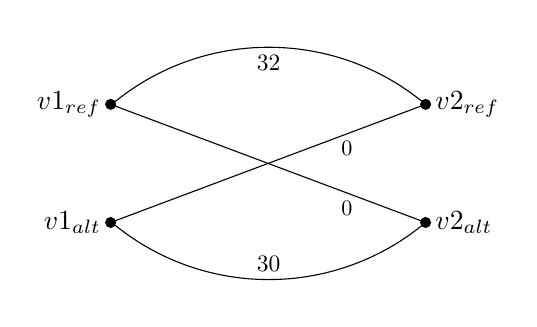
\begin{tikzpicture}[scale=1]
\def\xoffset{0}
\def\yoffset{0}

\def\titley{1.2}
\def\panellength{5}
\def\titlescale{1}
 \def\subtitlescale{0.7}
% \node[scale=\titlescale,align=center] at (0.5*\panellength+\xoffset,\titley+\yoffset){\textbf{a}. Phasing consistent in cis};

 \node[anchor=east] at (0 + \xoffset,2 + \yoffset) {$v1_{alt}$};
\draw (4 + \xoffset,2 + \yoffset) arc (-50:-130:3.1) node[midway,above, scale=0.85] {$30$};
\fill (0 + \xoffset ,2 + \yoffset) circle[radius=2pt];
\node[anchor=west] at (4 + \xoffset,2 + \yoffset) {$v2_{alt}$};
\fill (4 + \xoffset,2 + \yoffset) circle[radius=2pt];
\node[anchor=east] at (0 + \xoffset,3.5 + \yoffset) {$v1_{ref}$};
\fill (0 + \xoffset,3.5 + \yoffset) circle[radius=2pt];
\draw (4 + \xoffset,3.5 + \yoffset) arc (50:130:3.1) node[midway,below, scale=0.85]{$32$};
\draw (4 + \xoffset ,3.5 + \yoffset) -- node[below, scale=0.8] {$0$} (2 + \xoffset,2.75 + \yoffset) -- (0+ \xoffset,2 + \yoffset);
\draw (4 + \xoffset,2 + \yoffset) -- node[below, scale=0.8] {$0$} (2+ \xoffset,2.75 + \yoffset) -- (0+ \xoffset,3.5 + \yoffset);
\node[anchor=west] at (4+ \xoffset,3.5 + \yoffset) {$v2_{ref}$};
\fill (4+ \xoffset,3.5 + \yoffset) circle[radius=2pt];

\end{tikzpicture}\label{fig:a}}
\sidesubfloat[]{
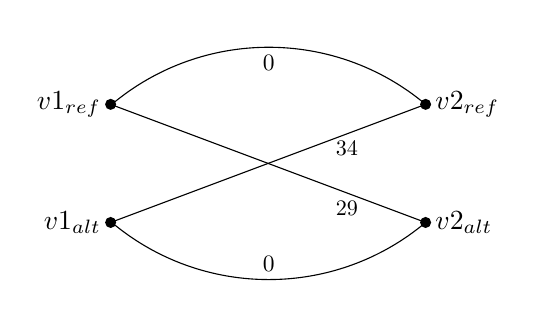
\begin{tikzpicture}[scale=1]
\def\xoffset{0}
\def\yoffset{0}

\def\titley{1.2}
\def\panellength{5}
\def\titlescale{1}
 \def\subtitlescale{0.7}
% \node[scale=\titlescale,align=center] at (0.5*\panellength+\xoffset,\titley+\yoffset){\textbf{a}. Phasing consistent in cis};

 \node[anchor=east] at (0 + \xoffset,2 + \yoffset) {$v1_{alt}$};
\draw (4 + \xoffset,2 + \yoffset) arc (-50:-130:3.1) node[midway,above, scale=0.85] {$0$};
\fill (0 + \xoffset ,2 + \yoffset) circle[radius=2pt];
\node[anchor=west] at (4 + \xoffset,2 + \yoffset) {$v2_{alt}$};
\fill (4 + \xoffset,2 + \yoffset) circle[radius=2pt];
\node[anchor=east] at (0 + \xoffset,3.5 + \yoffset) {$v1_{ref}$};
\fill (0 + \xoffset,3.5 + \yoffset) circle[radius=2pt];
\draw (4 + \xoffset,3.5 + \yoffset) arc (50:130:3.1) node[midway,below, scale=0.85]{$0$};
\draw (4 + \xoffset ,3.5 + \yoffset) -- node[below, scale=0.8] {$34$} (2 + \xoffset,2.75 + \yoffset) -- (0+ \xoffset,2 + \yoffset);
\draw (4 + \xoffset,2 + \yoffset) -- node[below, scale=0.8] {$29$} (2+ \xoffset,2.75 + \yoffset) -- (0+ \xoffset,3.5 + \yoffset);
\node[anchor=west] at (4+ \xoffset,3.5 + \yoffset) {$v2_{ref}$};
\fill (4+ \xoffset,3.5 + \yoffset) circle[radius=2pt];

\end{tikzpicture}\label{fig:b}
} \\

\sidesubfloat[]{
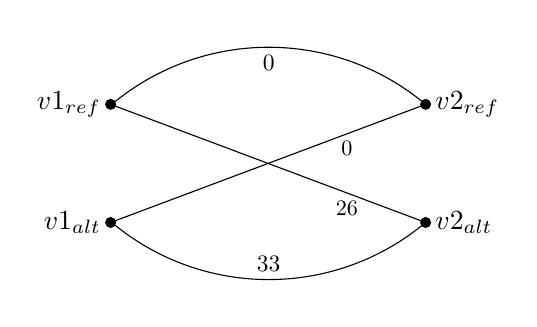
\begin{tikzpicture}[scale=1]
\def\xoffset{0}
\def\yoffset{0}

\def\titley{1.2}
\def\panellength{5}
\def\titlescale{1}
 \def\subtitlescale{0.7}
% \node[scale=\titlescale,align=center] at (0.5*\panellength+\xoffset,\titley+\yoffset){\textbf{a}. Phasing consistent in cis};

 \node[anchor=east] at (0 + \xoffset,2 + \yoffset) {$v1_{alt}$};
\draw (4 + \xoffset,2 + \yoffset) arc (-50:-130:3.1) node[midway,above, scale=0.85] {$33$};
\fill (0 + \xoffset ,2 + \yoffset) circle[radius=2pt];
\node[anchor=west] at (4 + \xoffset,2 + \yoffset) {$v2_{alt}$};
\fill (4 + \xoffset,2 + \yoffset) circle[radius=2pt];
\node[anchor=east] at (0 + \xoffset,3.5 + \yoffset) {$v1_{ref}$};
\fill (0 + \xoffset,3.5 + \yoffset) circle[radius=2pt];
\draw (4 + \xoffset,3.5 + \yoffset) arc (50:130:3.1) node[midway,below, scale=0.85]{$0$};
\draw (4 + \xoffset ,3.5 + \yoffset) -- node[below, scale=0.8] {$0$} (2 + \xoffset,2.75 + \yoffset) -- (0+ \xoffset,2 + \yoffset);
\draw (4 + \xoffset,2 + \yoffset) -- node[below, scale=0.8] {$26$} (2+ \xoffset,2.75 + \yoffset) -- (0+ \xoffset,3.5 + \yoffset);
\node[anchor=west] at (4+ \xoffset,3.5 + \yoffset) {$v2_{ref}$};
\fill (4+ \xoffset,3.5 + \yoffset) circle[radius=2pt];

\end{tikzpicture}\label{fig:c}}
\sidesubfloat[]{
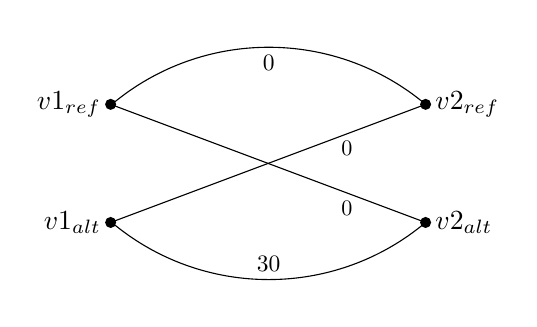
\begin{tikzpicture}[scale=1]
\def\xoffset{0}
\def\yoffset{0}

\def\titley{1.2}
\def\panellength{5}
\def\titlescale{1}
 \def\subtitlescale{0.7}
% \node[scale=\titlescale,align=center] at (0.5*\panellength+\xoffset,\titley+\yoffset){\textbf{a}. Phasing consistent in cis};

 \node[anchor=east] at (0 + \xoffset,2 + \yoffset) {$v1_{alt}$};
\draw (4 + \xoffset,2 + \yoffset) arc (-50:-130:3.1) node[midway,above, scale=0.85] {$30$};
\fill (0 + \xoffset ,2 + \yoffset) circle[radius=2pt];
\node[anchor=west] at (4 + \xoffset,2 + \yoffset) {$v2_{alt}$};
\fill (4 + \xoffset,2 + \yoffset) circle[radius=2pt];
\node[anchor=east] at (0 + \xoffset,3.5 + \yoffset) {$v1_{ref}$};
\fill (0 + \xoffset,3.5 + \yoffset) circle[radius=2pt];
\draw (4 + \xoffset,3.5 + \yoffset) arc (50:130:3.1) node[midway,below, scale=0.85]{$0$};
\draw (4 + \xoffset ,3.5 + \yoffset) -- node[below, scale=0.8] {$0$} (2 + \xoffset,2.75 + \yoffset) -- (0+ \xoffset,2 + \yoffset);
\draw (4 + \xoffset,2 + \yoffset) -- node[below, scale=0.8] {$0$} (2+ \xoffset,2.75 + \yoffset) -- (0+ \xoffset,3.5 + \yoffset);
\node[anchor=west] at (4+ \xoffset,3.5 + \yoffset) {$v2_{ref}$};
\fill (4+ \xoffset,3.5 + \yoffset) circle[radius=2pt];

\end{tikzpicture}\label{fig:d}
}

\par{
Example of a phasing consistent pair of heterozygous paired kmers \textbf{a)} in cis and \textbf{b)} in trans. \textbf{c)} shows an example of phasing inconsistency because the v2 kmer pair are not a heterozygous kmer pair, but because of paralogous sequence. The reference version of the v2 pair probably exists elsewhere in the genome. If this were due to a tandem repeat, we might expect all four edges to contain counts, perhaps with two edges having fewer counts due to fewer reads reaching into the 2nd repeat. \textbf{d)} shows a somewhat ambiguous case. From this, we do not know if v1 or v2 is heterozygous or not. This could arise from both being homozygous or one of them being heterozygous, but its pair not being the other haplotype.
}
\end{figure}

\par{
Figure \ref{figure:consistency2} show the main phasing consistent and inconsistent phenotypes for pairs of paired kmers. It is uncommon to get very mixed signals especially when working with HIFI data. When working with Hi-C data, pairwise counts are not of much use as it is rare for many Hi-C read pairs to link the same two heterozygous kmer pairs. Due to ambiguous cases that should be expected from data outlined in figure \ref{figure:consistency2}d, it is not always possible to categorize kmer pairs as heterozygous or paralogous from phasing consistency counts with one other kmer pair. We can then look across phasing consistency counts that a single kmer pair has with all of the kmer pairs with which it shares enough counts. In doing so we find some kmer pairs that are phasing consistent with some others and inconsistent with another set due to those other kmer pairs arising from paralogous sequence. And we also find kmer pairs which are inconsistent with all other kmer pairs because they were not truly heterozygous.
}



\subsection{Multiple heterozygous site haplotype phasing consistency}

\par{
When using phasing consistency as a signal for assembly scaffolding, we want to compare all heterozygous kmer pairs in one contig to all heterozygous kmer pairs in another contig. Figure \ref{figure:scaff} outlines what that looks like in the same way the previous phasing consistency diagrams did for pairs of individual kmer pairs. In order to do this, we will need to phase all heterozygous kmer pairs within each contig with respect to each other.
}

\begin{figure}[htbp!]
\caption{Phasing aware scaffolding}
\label{figure:scaff}
\begin{centering}
\includegraphics[width=\textwidth]{phasescaff.png}
\par{Using phasing consistency for scaffolding requires all of the heterozygous kmer pairs within a contig to already be phased with respect to one another.}
\end{centering}
\end{figure}



\subsection{\textit{de novo} haplotype phasing}

\par{
We use one or a combination of data types to do \textit{de novo} haplotype phase. The data type that is required is Hi-C, but long reads or linked reads can be used in addition to them. The reason Hi-C data is required is due to the very long range genetic information it gives us. With Hi-C, we are able to phase whole chromosomes instead of potentially having to break our phasing into phase blocks that are smaller than the chromosome. While there are existing phasing algorithms that can take multiple data types including Hi-C\cite{hapcut2}\cite{HICphasing}, we have developed our own phasing algorithm that has several benefits in general and to our specific purposes.
}

\subsubsection{Sparse \textit{Bernoulli} mixture model clustering}

\par{
We treat the haplotype phasing problem as a clustering problem. If we can cluster reads according to heterozygous kmer pair alleles they contain, this gives an implicit phasing of each kmer pair. Similar to the clustering algorithm in Chapter 2, we treat the haplotype clusters as vectors of allele fractions. Where in Chapter 2 this represented the probability parameter of a \textit{Binomial} because we were dealing with allele count data, here it will represent a \textit{Bernoulli} as we assume that a single read can only have one or the other of two alternate alleles. Of course each haplotype will only have one allele, but by treating it as a continuous number instead of a discrete number, we open the door to continuous numerical optimization methods which are often faster than discrete combinatorial optimization techniques. We let the optimization process allow the data to drive the allele fraction numbers to 0 or 1. 
}

\begin{figure}[htbp!]
\caption{Sparse \textit{Bernoulli} mixture model clustering haplotype phasing}
\label{figure:scaff}
\begin{centering}
\includegraphics[width=\textwidth]{sparsebernoulli.png}
\par{We treat the phasing problem as a sparse clustering problem in which we cluster reads into haplotypes.}
\end{centering}
\end{figure}

Definitions
\begin{itemize}
\item $H$: number of haplotypes. Lower case h will be used for indexing and referring to a specific haplotype.
\item $R$: number of reads. Lower case r will be used for indexing and referring to a specific read. 
\item $V$: number of kmer pairs. Lower case $v$ will be used to index and refer to a specific locus. We will assume only biallelic variants. $V_r$ will be a list of kmer pairs with observed data in read $r$.
\item $A$: Alleles. $A_{v,r}$ is a boolean representing whether read $r$ for kmer pair $v$ had the alternative allele or the reference allele.
\item $\phi_{h,v}$: cluster center value representing allele fractions of haplotype $h$ at locus $v$. We expect this to be near 1.0 or 0.0 because each haplotype can only have one allele or the other, but we allow the value to be continuous to allow for continuous numerical optimization techniques.
\end{itemize}

\noindent
\subsubsection{Model}

We use a maximum likelihood strategy by maximizing $\mathcal{L}(data)$ under a given model. 
\begin{equation}
\argmax_{\phi} \mathcal{L}(data, \phi)
\end{equation}


We define the likelihood of the data treating reads independently and marginalize each read across the haplotypes it could belong to. Each kmer pair is represented by a \textit{Bernoulli} with $\phi_{k,l}$ as the cluster center value representing the allele fraction for haplotype $h$ for kmer pair $v$.

Cluster model Likelihood function

\begin{equation}
\mathcal{L}(A) = \prod_{r \in R} \sum_{h \in H} \frac{1}{H} \prod_{v \in V_r} \begin{cases}       \phi_{h,v} & A_{v,r} == true \\      1 - \phi_{h,v} & A_{v,r} == false \\
\end{cases}
\end{equation}

\par{
We then maximize this likelihood with random initialization of haplotype cluster centers $\phi \in (0,1)$ with expectation maximization. A keen reader may note that due to the local nature of long reads and linked reads as well as the majority of Hi-C reads, this method can get stuck in local maxima in which for one region, the random initialization favored reads from one haplotype going to haplotype cluster 1 and in another region, reads from that same haplotype preferring haplotype cluster 2. In this case, the optimization would come into conflict at the boundary between these two regions. We could make this solve localized to a window and grow that window over time, but this would require knowledge of the assembly and make the method not truly \textit{de novo}. Or we could build our own graph and recruit new kmer pairs as we go. Another option is to use the very long scale Hi-C links for an initial solve, thus giving the haplotype cluster centers a rough global initial solve before adding in all of the data and fine tuning the local solutions. This also requires knowledge of the assembly making it not fully \textit{de novo}, but this is what we currently do. It is also possible that employing the same deterministic annealing strategy we did in Chapter 2, it may be able to get through these local maxima, but we have not tried this.
}
\subsubsection{Polyploid phasing}
\par{
This algorithm has several advantages to other haplotype phasing methods. While most methods scale super linearly, oftentimes exponentially, with ploidy if in fact they are able to solve polyploid phasing problems at all. In this method, since haplotypes are just cluster centers, we just add more cluster centers to match the ploidy. It would be untrue to say that this does not scale super linearly for an optimal solve. This algorithm does not guarantee optimality but neither do most of the modern phasing algorithms. The only modern phasing algorithm I know of which guarantees optimality is WhatsHap, a method which uses dynamic programming to preserve optimality but does not handle gapped data such as linked reads and Hi-C well\cite{whatshap}. So while our algorithm is not optimal, and its iterations to convergence may change with ploidy, the computation per expectation maximization step scales linearly with ploidy.
}
\subsubsection{Genotype correction via phasing}

\par{
Additionally our algorithm is highly robust to being given non heterozygous sites. Most phasing algorithms assume as input a set of heterozygous variants. However, even with standard resequencing, read mapping, and variant calling, some called variants will be false positives (also known as homozygous reference) or falsely called heterozygous when they are actually homozygous for the alternative allele. They could also be heterozygous or homozygous, but not with the stated alleles. This algorithm has the valuable property that we do not stipulate that every kmer pair is heterozygous. If they are not, the haplotype centers should be driven to the correct genotype by the data. If the reads support that this kmer pair is a false variant, the values will be driven to 0 for both haplotypes, and if the reads support the alternative on both haplotypes, the values will be both driven to 1. This type of genotype correction via phasing has been done before, but with a 3rd discrete categorical state on top of the two normal states representing a 0|1 vs 1|0 phasing\cite{mypatent}. In that method, the 3rd state represented either 0|0 or 1|1 by marginalizing across both. If that state was chosen, the posterior for each case was calculated and genotype reassigned accordingly. This does work, but has the dramatic downside of increasing the total solution space from $2^n$ to $3^n$.
}


\begin{figure}[htbp!]
\caption{Sparse \textit{Bernoulli} mixture model phasing allows for polyploid phasing and genotype correction}
\label{figure:bernoulli}
\begin{centering}
\includegraphics[width=\textwidth]{poly.png}
\par{In order to handle polyploid phasing, we simply increase the number of cluster centers. And because we do not stipulate that every site is heterozygous, the algorithm can naturally correct miscalled genotypes.}
\end{centering}
\end{figure}


\par{
We ran this algorithm on Hi-C, linked read, and HIFI data from a butterfly \textit{Vanessa atalanta} from the Darwin Tree of Live (DToL) project. We then compare this phasing to which allele the HiCanu assembly 
contained. Initially we show the phasing cluster center values on a single contig to compare phasing with Hi-C alone vs with linked reads and/or long reads (see figure \ref{figure:hicphasing1}.
}

\begin{figure}[htbp!]

\caption{Phasing with Hi-C alone vs combined data}
\label{figure:hicphasing1}
\begin{centering}
\includegraphics[width=\textwidth]{hicphasing1.png}
\par{Here we show the haplotype cluster center values for sparse \textit{Bernoulli} mixture model haplotype clustering with the values for the haplotype 2 cluster offset by -0.2 such that any phase switches would be visible and not overwritten by other data points. We see that Hi-C alone produces fairly noisy phasing probably because the chances that a HI-C read hits two heterozygous loci it fairly low reducing the total amount of useful data. When linked reads and/or HiFi reads are added, the phasing becomes much cleaner.}
\end{centering}
\end{figure}


\par{And in figure \ref{figure:hicphasing2} we show the phasing against the entire genome.

\begin{figure}[htbp!]

\caption{Phasing whole \textit{Vanessa atalanta} genome}
\label{figure:hicphasing2}
\begin{centering}
\includegraphics[width=\textwidth]{hicphasing2.png}
\par{Phasing for whole \textit{Vanessa atalanta} genome. Here you can see that contig 1 as well as the first and last large contigs on the last row are sex chromosomes and thus haploid. Again, the cluster center values for haplotype cluster 2 were offset down by 0.2 for visibility. And contigs are split across multiple rows for better visibility. We can see here rare, but notable long switch errors vs the HiCanu assembly. Because we are using Hi-C data with chromosome length scale information, it is highly likely that these phase switch errors are errors in the assembly and not our phasing algorithm. }
\end{centering}
\end{figure}

\subsection{Phasst phase: Reference or assembly based phasing}

\par{
Because the sparse \textit{Bernoulli} mixture model haplotype phasing can run into local optima because of the local nature of most read types, it currently requires plentiful and high quality Hi-C data. Also, for some organisms, such as diptera, chromosome pairs colocate within the nucleus\cite{somaticpairing}, greatly increasing the number of cross haplotype Hi-C links. This makes it not always sufficient to have an initial solve with just the long range Hi-C. We still believe that that algorithm can be made to work either with a moving or expanding window or through deterministic annealing, but we decided to take another direction for the time being. So we developed a reference/assembly based phasing consistency rules based phasing algorithm. We first find a good seed kmer pair by looking at all pairwise phasing consistencies. The kmer must have sufficient other kmers that it is phasing consistent with. Then we add phasing consistency counts for all molecules that contain this seed kmer pair to a growing data structure and mark those molecules as used. We also create a priority queue of kmer pairs according to the HiFi reads taking into account reverse compliment such that we are only adding kmers in one direction. Then, at each step, we pop the front kmer pair off of the priority queue and assess its phasing consistency counts. If they are sufficiently phasing consistent (>90\% cis or trans, minor allele fraction of >15\%, >10 total phasing consistency counts), we add that kmer pair to the growing phase block in the appropriate phase (whether its dominant counts were cis or trans). And we then look at all molecules containing that kmer pair, and, if not marked as used, update phasing consistency counts for other kmer pairs those molecules contain and then mark those molecules as used. If the kmer pair is not sufficiently phasing consistent, we mark it as used and unphased and continue. We proceed in this manner until the priority queue is empty. We then reseed at the initial seed and add kmer pairs to the priority queue in the opposite direction, keeping track of phasing consistency counts and building the phase block in the other direction until we can no longer continue. For this step we use both the HiFi and linked reads, both of which have a very low error/cross haplotype signal. Only the HiFi data is used to build the priority queue as the linked reads don't have direction across different reads within the same barcode.
}

\begin{figure}[htbp!]
\caption{Building phase blocks}
\label{figure:phaseblocks}
\begin{centering}
\includegraphics[width=0.6\textwidth]{phaseblockbuilding.png}
\par{Diagram outlining the process of building phase blocks with HiFi and linked reads using phasing consistency rules. }
\end{centering}
\end{figure}

\par{
Because we have only used HiFi reads and linked reads in the process thus far, we do not expect to be creating contig or chromosome length phase blocks. Instead, we make very high quality phase blocks that we can then phase with respect to one another using the Hi-C reads. This is very similar to how we will use Hi-C for phasing aware scaffolding in the sections to come. We simply look at all Hi-C reads, and for ones that have two or more phased kmer pairs in different phase blocks, we add them to the inter-phaseblock phasing consistency counts. Because the phase blocks should be of a reasonable length (hundreds of kb), there are plenty of Hi-C molecules linking them with two or more heterozygous kmer pairs.
}

\par{
We ran this on the same data, this time using the HiCanu assembly post purge dups but pre-scaffolding and curation.
}


\begin{figure}[htbp!]
\caption{Phasst phase results on \textit{Vanessa atalanta}}
\label{figure:phasstphase}
\begin{centering}
\includegraphics[width=\textwidth]{phasstphase.png}
\par{Phasst phase shows cleaner phasing than sparse \textit{Bernoulli} mixture model phasing because it skips over any kmer pairs that are not phasing consistent, it only allows discrete phasing instead of a continuous solution, and sex contigs have been detected and skipped. }
\end{centering}
\end{figure}

\subsection{Haploid / sex contig detection}

\par{
We want to only use phasing consistency when it should be expected to work---when the chromosome is diploid (or polyploid if we extended these rules to apply to polyploid genomes). This makes contigs coming from haploid sex chromosomes problematic. So we would like to detect these prior to phasing and scaffolding such that we can treat them separately in a more standard fashion of just using Hi-C read linkage as a signal for scaffolding. We use kmer counts and kmer pair density as signals for diploid contigs. Using a fast kmer package from Gene Myers called FASTK \cite{fastk}, I find all kmers that occur exactly once in the assembly and check their counts in the HiFi data and take the mean for each contig. For kmer pair density, I simply find how many of the kmer pairs occur on each contig and divide by the contig length. Figure \ref{figure:sexcontigs} shows contig kmer counts vs kmer pair density for \textit{Vanessa atalanta} for contigs > 100kb.
}

\begin{figure}[htbp!]
\caption{Haploid / sex contig detection for \textit{Vanessa atalanta}}
\label{figure:sexcontig}
\begin{centering}
\includegraphics[width=0.65\textwidth]{sexcontig.png}
\par{Kmer counts are a signal for haploid/sex contigs, but only a weak one because the heterozygosity for this species is so large, much of the sequencing in diploid chromosomes are haploid counts. Kmer pair density is a much better signal for haploid contigs. The three contigs on the left of the graph are sex contigs. The one intermediate contig is just over 100kb and we do not know if it is diploid or not. }
\end{centering}
\end{figure}

\par{
While haploid sex contig detection works well for this dataset and assembly, it is quite different for different species. This could be due to pseudo autosomal regions, repeat structure, or several other factors. In general it is best to use orthologous genes known to be on sex chromosomes in related species for sex contig detection.
}

\subsection{Contig breaking}

\par{
Before scaffolding, we want to break any contigs which are likely chimeric misassemblies. This is a common first step in scaffolding \cite{SALSA}\cite{scaffoldingreview}. We use the Hi-C data links to break contigs across regions where there is extremely low or no Hi-C links. We use both paired kmers as well as a sampling of likely homozygous kmers in order to utilize more of the data. We have a sweeping window of kmer positions on the contig and count how many Hi-C links cross the midpoint of that window. We keep track of all counts and the phasing consistency counts of kmer pairs across the midpoint of the window separately. Figure \ref{figure:contigbreaking} shows a depiction of this process as well as data on a contig which contains a chimeric misassembly and requires breaking from the \textit{Vanessa atalanta} HiCanu assembly. We show both total links across the midpoint of a 200 kmer pair window as well as the percent phasing consistency across that window. In this case, the total links drops to zero, so of course the phasing consistency also drops to zero, but you can see how phasing consistency for breaking contigs can be a very powerful signal. However, this does require that you have detected the sex contigs and treat them differently. With this, we find the same three breaks in the HiCanu assembly that SALSA does.
}

\begin{figure}[htbp!]
\caption{Contig breaking using Hi-C total linkage and phasing consistency}
\label{figure:contigbreaking}
\begin{centering}
\sidesubfloat[]{
\includegraphics[width=0.75\textwidth]{contigbreaksdiagram.png}
} \\
\sidesubfloat[]{
\includegraphics[width=\textwidth]{contigbreaksdata.png}
}
\par{\textbf{a)} shows the setup for contig breaking. We work in a 200bp window and look at linkage and phasing consistency across the midpoint of a sliding window. Below, \textbf{b)} shows the results of this at each position of that sliding window. }
\end{centering}
\end{figure}


\section{Pedigree sample strategies}
As discussed already there are simple strategies for splitting long reads by haplotypes using short accurate reads from both parents. 
But for many species such as wild caught samples it may be difficult to obtain the paternal sample whereas it is possible to capture a 
fertilized female and grow her brood in isolation. For this case we propose to use three short read samples: one maternal sample, one sample 
from a single F1, and another sample from a pool of multiple F1 offspring. From these samples we can obtain distinguishing kmers or probabilistic 
distinguishing kmers for each haplotype of both the mother and father.

\begin{figure}[h!]
\caption{Pseudotrio}
\label{figure:pseudotrio}
\begin{centering}
\includegraphics[width=\textwidth]{pseudotrio.png}
\end{centering}
\end{figure}

As shown in \ref{figure:pseudotrio} we can obtain distinguishing kmers for the P1 haplotype by set subtraction of kmers in the maternal and single F1 sample 
from the those in the pooled samples. In a similar way we can subtract kmers in the maternal sample from the single F1 sample to get probabilistic distinguishing 
kmers from the P2 haplotype. We say probabilistic distinguishing kmers because these kmers could also occur on the P1 haplotype as well. And in the same way 
we can get probabilistic distinguishing kmers for the M1 haplotype by subtracting kmers in the single F1 sample from those in the maternal sample. And finally we can obtain 
probabilistic distinguishing kmers for the M2 haplotype will be obtained by selecting kmers which are shared between the maternal and single F1 sample and occur at 
haploid counts in both samples. Once we have these distinguishing kmers we can use them to separate long reads by haplotype for libraries created from any of these samples. 
We have created software for collecting these distinguishing kmers \cite{distinguishing_kmers} which uses counting bloom filters to minimize memory usage 
and a mod based system allowing distribution of jobs to many worker nodes. And we also have software for binning long reads based on those 
distinguishing kmers \cite{long_read_binner}.


\section{Phasstools: phasing and assembly tools}
\subsection{Heterozygous kmer pairs and detection}
First we tackle the subject of identifying heterozygous variants in a reference-free manner. We will do this using a kmer approach, as many reference-free methods do. 
Many people have focused on identifying kmers which occur at roughly half counts in short read data \cite{KAT} and various software exists to count kmers \cite{jellyfish} 
and to model the mixture of expected distributions (errors, haploid, diploid, duplication kmers) \cite{genomescope}. Identifying heterozygous kmers in this way 
suffers from multiple problems from the perspective of de novo phasing. 1. Many of these identified as half counts will be either randomly high count error kmers or randomly low count 
homozygous kmers. 2. You end up with $K-1$ overlapping kmers for a given variant which is needlessly redundant information which will both slow down any phasing algorithm and 
likely break key independence assumptions. And 3. while you have heterozygous kmers, you don't know which kmers are alternative alleles of each other. 
We propose finding pairs of kmers which vary only in the center position which are also both roughly at half counts. These heterozgyous SNP kmers 
will be much more robust and have the benefit of knowing that one is the alternative allele of the other.
We have software for this purpose \cite{het_kmers} which uses counting bloom filters to minimize memory usage and a mod based method to 
distribute the work to many worker nodes.

\subsection{Phasst scaff: phasing aware assembly scaffolding}

\par{
Now that we have the paired kmers phased on each contig, at least for the ones that could be phased, we can now look at the phasing consistency counts of pairs of contigs by looking at Hi-C reads that contain kmer pairs that occurs on two contigs. An example of a phasing consistent match we found has the following counts:  cis1: 10150, cis2: 10278, trans1: 98, trans2: 101. We do a binomial test to compare cis vs trans counts to a random expectation of 0.5 and of course these numbers yield exceedingly low p-values. The counts between non matches are essentially randomly distributed between cis and trans. For the HiCanu assembly of the butterfly \textit{Vanessa atalanta}, we find the same scaffolding matches that SALSA2 finds.
}

\subsubsection{Chromosome binning}

\par{
Using these matches, we create a graph where nodes are contigs and edges are phasing consistent scaffolding matches. We find the connected components of this graph which represent the chromosomes these contigs belong to. 
}

\subsubsection{Order and orientation}

\par{
To order and orient, we take the heterozygous and homozygous kmers on the ends of each contig (100,000 bases on each contig end, or to the middle of the contig), and count how many Hi-C reads link the start and end of each contig to the start and end of each other contig in the chromosome bin. We normalize this number by the actual length used (if less than 100,000). The next part, I have not completed, but I will describe the plan and how it differs from what is currently done. Essentially, SALSA takes these normalized link numbers between the ends of each contig that passes its scaffolding thresholds and takes the highest weight link and makes that a new longer scaffold and then the next highest weight until completion. We intend to create a stochastic process in which we choose our edges with some probability weighted on the normalized linkage value and otherwise proceed as SALSA does. We will then run this process many times and choose the final scaffolding that maximizes the total sum of normalized linkage weights. We can also then report for each link, in how many of the simulated scaffoldings were those contigs connected in that way to give a level of confidence to the ordering and orientation.
}

\subsection{Phasst a: phased assembly}

\par{
Our first attempt at phased assembly simply used pairwise phasing consistency of kmer pairs. We created a graph where kmer pairs are nodes and edges exist if the two kmer pairs are phasing consistent. We made an edge between two kmer pairs if the phasing consistency was >90\%, minor edge of the major phasing was >15\%, and there were at least 10 total counts. This creates megabase scale graphs that are linear on a global level. Figure \ref{figure:phasegraph} shows examples of these graphs visualized in Gephi with graph layout force atlas 2\cite{gephii}\cite{forceatlas2}. 
}

\begin{figure}[htbp!]
\caption{Example phasing consistency graph contigs for \textit{Vanessa atalanta}}
\label{figure:phasegraph}
\begin{centering}
\includegraphics[width=\textwidth]{phasinggraph.png}
\par{Graph of kmer pairs with edges between them if they are phasing consistent. }
\end{centering}
\end{figure}

\par{
The idea is to then use this phasing consistency graph as psuedo contigs from which we could then phase these kmer pairs, and then bin reads into contig bins and haplotype bins within those contigs and do haploid assembly of those reads. Unfortunately, not all of these graphs were globally linear. This meant that we had some incorrect edges. Increasing the stringency of the phasing consistency thresholds did not get rid of all of these spurious connections. If we proceeded with this plan, this could lead to chimeric misassemblies. Figure \ref{figure:misassemblygraph} shows two examples of these misassembly causing connections.
}

\begin{figure}[htbp!]
\caption{Example of errors in phasing consistency graph for \textit{Vanessa atalanta}}
\label{figure:misassemblygraph}
\begin{centering}
\includegraphics[width=\textwidth]{misassemblyphase.png}
\par{Errors in misassembly graph. On the left we see an error in which a single kmer pair is phasing consistent with another single kmer pair elsewhere in the genome. This type of error reduces as the phasing consistency thresholds are made more striict, but the resulting graph becomes more and more fractured. On the right, we see a single kmer pair consistent with many kmer pairs in two locations. This is because this kmer pair is truly heterozygous in both locations in the genome. This error mode does not reduce with further stringency. }
\end{centering}
\end{figure}

\subsubsection{Phasing consistent heterozygous kmer recruitment}
\subsubsection{Haplotype and chromosome read binning}
\subsubsection{Haploid chromosome assembly}



\section{Discussion}

